
\documentclass[a4paper]{report}
\usepackage[utf8x]{inputenc}
% bibliography
\usepackage{natbib}
%\bibpunct{[}{]}{,}{a}{}{;}

\usepackage{fancyheadings}
\usepackage{iamdip}
\usepackage[pdftex]{graphicx}
% ignore missing images
%\usepackage[demo]{graphicx}
\usepackage[labelfont=bf, font={sf,normalsize}, margin=0.5cm]{caption}
\usepackage{caption}
\usepackage{subcaption}
\usepackage{amsmath}
\usepackage{marvosym}
\usepackage{amssymb}
\usepackage{amsfonts}
\usepackage{url}
\usepackage{hyperref}
\usepackage[procnames]{listings}
\usepackage{chngpage}
\usepackage{rotating}
\usepackage{wrapfig}

% For notation table
\usepackage{tabulary}
\usepackage{booktabs}

\usepackage{here}

\headrulewidth 0.5pt \addtolength{\headheight}{5pt}
\lhead[\fancyplain{}{\rm\thepage}]{\fancyplain{}{\rightmark}}
\rhead[\fancyplain{}{\leftmark}]{\fancyplain{}{\rm\thepage}}
\cfoot{}

\graphicspath{{Figures/}}

\newcommand{\T}{^\text{T}}

% for fancy todo
\usepackage{todonotes}
\newcommand{\todoRef}{\todo[color=green!20]}
\newcommand{\todoEnglish}{\todo[color=red!20]}
\newcommand{\todoFormat}{\todo[color=blue!20]}
\newcommand{\todoWriteMore}{\todo[color=yellow!40, inline]}
\newcommand{\todoRewrite}{\todo[color=purple!20, inline]}
\newcommand{\todoQ}{\todo[color=blue!20]}

% math definitions, propositions and such
\usepackage{amsthm}
\newtheorem{definition}{Definition}
\newtheorem*{rules}{Rules}
\newtheorem*{example}{Example}
\newtheorem*{assertion}{Assertion}

% tree packages and basic settings
\usepackage{tikz}
\usetikzlibrary{arrows,shapes,positioning,shapes.geometric,fit}
\usepackage{xcolor}
\tikzset{
treenode/.style = {align=center, inner sep=0pt, text centered,
font=\sffamily},
arn_n/.style = {treenode, circle, white, font=\sffamily\bfseries, draw=black,fill=black, text width=1.5em},% arbre rouge noir, noeud noir
arn_r/.style = {treenode, circle, black, draw=blue, text width=1.5em, very thick},% arbre rouge noir, noeud rouge
arn_w/.style = {treenode, circle, draw=black, text width=1.5em, very thick},% arbre rouge noir, noeud rouge
arn_x/.style = {treenode, rectangle, draw=black, minimum width=0.5em, minimum height=0.5em},% arbre rouge noir, nil
subtree/.style  = {regular polygon, regular polygon sides=3, draw=black, align=center, minimum size=1cm, anchor=center}
}

\newcommand{\newCommandName}{text to insert}
%%%%%%%%%%%%%%%%%
% begin document
\begin{document}

\pagestyle{fancyplain} \thispagestyle{empty}

\title{A Proof Search Implementation in Python\\ for Justification Logic}
\author{Judith Fuog}
\betreuer{Prof.\ Dr.\ Thomas Studer}
\ort{Bern}
\datum{2015}


\pagenumbering{roman} \setcounter{page}{1}
\maketitle

\newpage
\thispagestyle{empty}
\vspace{8cm}
\noindent
{\centerline {\bf \large Abstract}}
\vspace{1cm}
\label{abstract}
%!TEX root = ../bachelors_thesis.tex

Justification Logic as part of the larger field modal logic provides some means to give more information about a proof. Information and researches about this topic are currently still rather limited. 

However the thesis presented here does not concern itself with the theoretical details of Justification Logics but focus on a proof search approach for this specific logic.  The implementation is done in the language Python.

\pagenumbering{roman} \setcounter{page}{1}
\tableofcontents


\newpage{\pagestyle{empty} \cleardoublepage}

% Hauptdokument
\pagenumbering{arabic} \setcounter{page}{1}
\pagestyle{fancy}


\chapter{Introduction}
\section{Motivation}
\section{Goal}
\section{Overview}



\chapter{Justification Logic}
\label{chap: Justification Logic}
%!TEX root = ../bachelors_thesis.tex
The theory of Justification Logic as it is used here requires little knowledge of the wide fields of Modal Logic apart from some very basic knowledage about logic theory. For the purpose of this proof search a few basic rules and definitions are sufficient to provide the needed knowledge. 
\par

 The theory presented here is oriented mainly on the work of \cite{goet} as well as the older reference \cite{art} and also from the homepage \cite{stan}. This definitions and rules given here are not complete to the justification logic. Priority was given to those informations which are vital for the implementation. So however briefly and incomplete the theory is presented here full reference can be found in the named sources. 

\section{Background}
Justification Logic has its origins from the field of modal logic. 
In model logic $\square A$ means that $A$ is \emph{know} or that we have \emph{proof} of $A$. In justification logic the equivalent would be $t:A$ where $t$ is a \emph{proof term} of $A$. This provides us the notion that \emph{knowledge} or \emph{proofs} may come from different sources. Justification logic lets us connect different \emph{proofs} with a few simple operators and thus give us a better desciption of the proof. It may be said that where in model logic the knowledge is implicit it is explicit in Justification Logic\footnote{\cite{goet}}.

\section{Rules and Definitions}

The language of justification logics is given here in a more traditional format with falsum and implication as primary propositional connectives. Although for the work done with this implementation only the implication has been used and the falsum has been ignored. \footnote{cite here! S. 17} Also not all available syntactic objectes are introduces here but only those implemented.

\begin{definition}\label{justification_terms} Apart from formulas, the language of justification logics have another type of syntactic objects called \emph{justification terms}, or simply \emph{terms} given by the following grammar:
\[
	t::= c_{i}^{j} | x_i | \bot | (t \cdot t) | (t+t) | !t
\]
where $i$ and $j$ range over positive natural numbers, $c_{i}^{j}$ denotes a (justification) \emph{constant} of level $j$, and $x_i$ denotes a (justification) \emph{variable}.

The binary operations $\cdot$ and $+$ are called \emph{application} and \emph{sum}. The unary operation $!$ is called \emph{positive introspection}.
\end{definition}

\begin{rules}\label{rules} 

\begin{itemize} Application, sum and positive introspection respectively.

	\item[C1] $t:(F \rightarrow G, s:F \vdash t \cdot s: G$
	\item[C2] $t:F \vdash (t +s):F, \:\: s:F \vdash (t+s):F$
	\item[C3] $t:F \vdash !t:t:F$
\end{itemize}

\end{rules}

Formulas are constructed from propositional letters and boolean constants in the usual way with an additional clause: if $F$ is a formula dn $t$ a term, then $t:F$ is also a formula.

\begin{definition}\label{justification_formulas} \emph{Justification formulas} are given by the grammar:
\[
A ::= P_i|(A \rightarrow A) | (t:A)
\]
where $P_i$ denotes a proposition, as in the modal language, and $t$ is a justification term in the justification language.
\end{definition}

This is almost all we need for the proof search of a (justification) formula. The last definition gives us something like a reference for the proof constants.

\begin{definition}\label{cs-def} A constant specification, \emph{CS}, is a finite set of formulas of the form $c:A$ where $c$ is a proof constant and $A$ is a axiom of Justification language.
\end{definition}

The axioms mention in this definition are \emph{C1-C3} in addition to $t:F \rightarrow F$ and the Axioms of the classical propositional logic in the language of LP.



\newpage{\pagestyle{empty} \cleardoublepage}

\chapter{A Divide and Conquer Algorithm}
\label{chap: Algorithm A Divide and Conquer Approach}
%!TEX root = ../bachelors_thesis.tex
\section{The Core Idea}
In my earliest attempts the methods of my algorithm had the tendency to explode with the number of \texttt{if-else} and \texttt{switch} statements. Also they were always very deep nestled. It was sheer impossible to keep track of what had to be done where under which circumstances and whenever I though I had it I found more cases that needed takes special care of. What I really needed was a strategy. I started experiencing with the proof terms of the justification formula, trying to take it somehow apart and restructure the formula in a way that would make handle it easier. I was looking for something like the conjunctive normal form (CNF) and the way how it is used in proof search calculus\footnote{\emph{Proof Search Calculus} as it is introduced by Jäger \cite{jaeg}.}. Indeed I found a way that allows me to \emph{divide} a justification formula in disjunctive formulas where proving only one of them is also proof for the whole justification formula. The main advantage gained from dividing the justification formula is that the resulting formula have far less variety in the manner of their operations and thus are easier to further analyze.

The comprehension that my approach follows a classic \emph{Divide and Conquer} approach came to me only later when I started \emph{conquering}. The algorithm presented here may not be a model of \emph{Divide and Conquer} but similarities cannot be denied. For that reason I have structured this chapter accordingly.

\medskip

There are two major steps in the divide part of this algorithm. First the justification formula itself will be split into several smaller pieces and adjusted. Second each of those smaller pieces called \emph{atoms} is also being be taken apart so that only their proof constant with a corresponding proof term containing variables remains. The pair of proof constant and proof term will be called \emph{must}\footnote{They are called \emph{musts} in the algorithm because we have to find a match for every single one of them or else the atom is not provable.}.

The conquer step first handles the \emph{musts} of one atom, trying to find a valid match for every \emph{must} in the constant specification list and then evaluates from the results of each \emph{atom} the provability of the originally given justification formula.

\section{Divide}\label{chap:Algorithm.divide}
The aim of this first step is to split it into smaller pieces and standardize them to make it easier to get the \emph{musts}.

\subsection{Atomize a Justification Formula}\label{chap:Algorithm.atomize}
\begin{definition}[atomic]
	A formula or term is called \textbf{atomic} if it fulfills the following conditions:
	\begin{itemize}
		\item The term contains no sum operations.
		\item A introspection operation can neither be the top operation of a term nor be the left operant of a application operation.
	\end{itemize}	
\end{definition}
To make the content presented here more understandable the following example will illustrate the steps taken.\footnote{It is on purpose that the \emph{justification term} is by far more complicated than statement $b:F$ that follows the \emph{justification term}. As far as this algorithm goes the complexity of the statement is of no further consequence and thus is kept as simple as possible to allow a easier overview.}

\subsubsection{Sumsplit}
\label{sumsplit}
From the sum rule of justification logic in \ref{rules} it follows that checking for provability in a formula where the top operation is a sum is equal to checking either operant of the sum and if any of it is provable so is the original formula.

\begin{align}\label{ss1}
	(s+t):F \quad \Rightarrow \quad s:F \lor t:F
\end{align}

%!TEX root = ../bachelors_thesis.tex
\begin{figure}[H]
\begin{center}
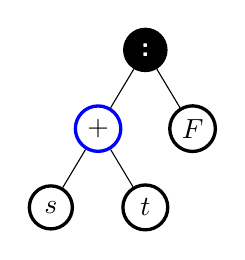
\begin{tikzpicture}[level distance=1cm,
  level 1/.style={sibling distance=1.2cm}]
	\node [arn_n]{:}
	  child {node [arn_r]{\(+ \)}
	  	child {node [arn_w] {$s$}}
	  	child {node [arn_w] {$t$}}
	  }
	  child {node [arn_w]{$F$}};
\end{tikzpicture}
\hspace{2cm}
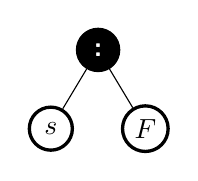
\begin{tikzpicture}[level distance=1cm,
  level 1/.style={sibling distance=1.2cm}]
	\node [arn_n]{:}
	  child {node [arn_w]{\(s\)}}
	  child {node [arn_w]{$F$}};
\end{tikzpicture}
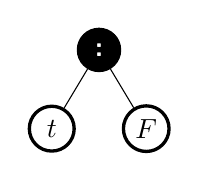
\begin{tikzpicture}[level distance=1cm,
  level 1/.style={sibling distance=1.2cm}]
	\node [arn_n]{:}
	  child {node [arn_w]{\(t \)}}
	  child {node [arn_w]{$F$}};
\end{tikzpicture}
\caption{Example of a simple sumsplit.}
\end{center}
\end{figure}

This is also true for formulas where sum is not the top operation. Here $X$ denotes a arbitrary \emph{justification term}.

\begin{align}\label{ss2}
	(r*(s+t)):F  \quad & \Rightarrow r: X \rightarrow F \land (s+t): X \\
	& \Rightarrow ( r: X \rightarrow F \land s: X ) \lor ( r: X \rightarrow F \land t: X )
\end{align}

%!TEX root = ../bachelors_thesis.tex
\begin{figure}[H]
\begin{center}
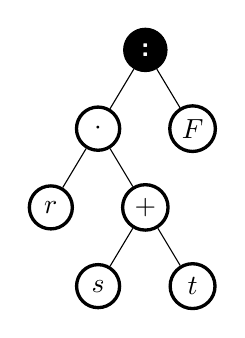
\begin{tikzpicture}[level distance=1cm,
  level 1/.style={sibling distance=2cm},
  level 1/.style={sibling distance=1.2cm}]
	\node [arn_n]{:}
	  child {node [arn_w]{\(\cdot \)}
	  	child {node [arn_w] {$r$}}
	  	child {node [arn_w] {$+$}
		  	child {node [arn_w] {$s$}}
		  	child {node [arn_w] {$t$}}	  		
	  	}
	  }
	  child {node [arn_w]{$F$}};
\end{tikzpicture}
\hspace{1.5cm}
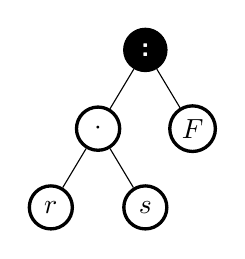
\begin{tikzpicture}[level distance=1cm,
  level 1/.style={sibling distance=1.2cm}]
	\node [arn_n]{:}
	  child {node [arn_w]{\(\cdot \)}
	  	child {node [arn_w] {$r$}}
	  	child {node [arn_w] {$s$}}
	  }
	  child {node [arn_w]{$F$}};
\end{tikzpicture}
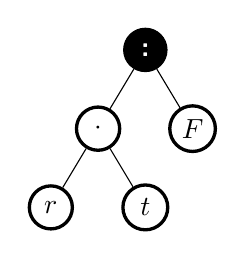
\begin{tikzpicture}[level distance=1cm,
  level 1/.style={sibling distance=1.2cm}]
	\node [arn_n]{:}
	  child {node [arn_w]{\(\cdot \)}
	  	child {node [arn_w] {$r$}}
	  	child {node [arn_w] {$t$}}
	  }
	  child {node [arn_w]{$F$}};
\end{tikzpicture}
\end{center}
\caption{Example of a sumsplit where the sum is not the top operation.}
\end{figure}

\subsubsection{Simplify Introspection}
In this step we try to get rid of any introspection operation that is the first operation of a formula. Either the introspection can be removed and the formula simplified or else the formula is not provable at all and can be discarded.

Derived from the application rule in \ref{rules} we get the following:

\begin{align}\label{sb}
	!t:(t:F) \quad & \Rightarrow t: F
\end{align}

%!TEX root = ../bachelors_thesis.tex
\begin{center}
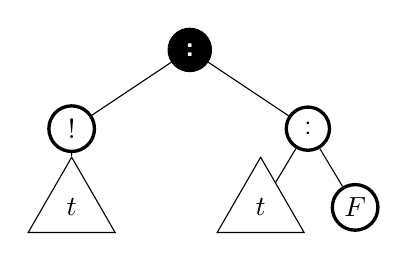
\begin{tikzpicture}[level distance=1cm,
  level 1/.style={sibling distance=3cm},
  level 2/.style={sibling distance=1.2cm}]
	\node [arn_n]{:}
	  child {node [arn_w]{\(! \)}
	    child[right] {node [subtree] {$t$}}
	    }
	  child {node [arn_w]{:}
  		child {node [subtree] {$t$}}
  		child {node [arn_w] {$F$}}
  		};
\end{tikzpicture}
$\Longrightarrow$
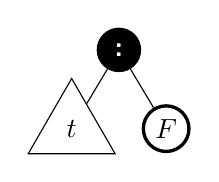
\begin{tikzpicture}[level distance=1cm,
  level 1/.style={sibling distance=1.2cm}]
	\node [arn_n]{:}
	  child {node [subtree]{\(t \)}}
	  child {node [arn_w]{$F$}};
\end{tikzpicture}
\end{center}

Speaking in the manner of a syntax tree it needs to be checked, if the child of the introspection operation is identical with the left child of the right child of the root. In that case the formula can be simplified to right child of the root only. Else there is no way to resolve the introspection operation and the formula has to be discarded.

\subsubsection{Remove Contradicting Introspection}
This last step in atomizing the formula proved to be on of the hardest to realize. Only countless examples support the claim that the introspection operation must not be the direct left child of a application operation. In coming to that conclusion it has been helpful that no sum operation could make the situation more complex. Because of this and also the fact that a introspection operation is never the top operation in a formula it is guarantied that a introspection operation must be either a right child or a left child of a application operation.

\begin{align}\label{bb}
	((!s)\cdot t):F  & \Rightarrow \exists X_1 : ((!s): (X_1 \rightarrow F) \; \land \; t: X_1)\\
	(!s): (X_1 \rightarrow F)  &\Rightarrow \exists X_2 : ((X_1 \rightarrow F) = (s:X_2)) & \text{\Lightning}
\end{align}
The last line gives a contradiction since there is no possible $X_2$ that would fulfill the condition of $X_1 \rightarrow F = s:X_2$.

\begin{assertion}[Tree Version]
A introspection operation that is the direct left child of a application operation causes the whole term to be invalid (unprovable), given that the term is without sum operations and no introspection operation at the top.
\end{assertion}

%!TEX root = ../bachelors_thesis.tex
\begin{figure}[H]
\begin{center}
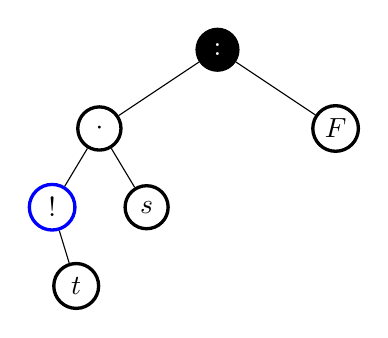
\begin{tikzpicture}[level distance=1cm,
  level 1/.style={sibling distance=3cm},
  level 2/.style={sibling distance=1.2cm}]
	\node [arn_n]{$:$}
	  child {node [arn_w]{\(\cdot \)}
	    child {node [arn_r] {$!$}
	    		child[right] {node [arn_w] {$t$}}
	    	}
	    child {node [arn_w] {$s$}}
	    }
	  child {node [arn_w]{$F$}};
\end{tikzpicture}
\hspace{2cm}
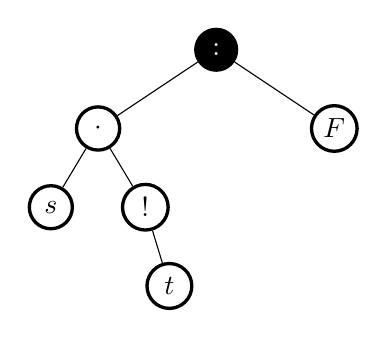
\begin{tikzpicture}[level distance=1cm,
  level 1/.style={sibling distance=3cm},
  level 2/.style={sibling distance=1.2cm}]
	\node [arn_n]{$:$}
	  child {node [arn_w]{\(\cdot \)}
	    child {node [arn_w] {$s$}}
	    child {node [arn_w] {$!$}
	    		child[right] {node [arn_w] {$t$}}
	    	}
	    }
	  child {node [arn_w]{$F$}};
\end{tikzpicture}
\end{center}
\caption{The left tree shows an introspection that gives a contradiction, while the right tree is valid.}
\end{figure}

This concludes the \emph{atomization} of one formula to many simple formulas which can be checked for provability individually. An atomized formula now consists only of application operations and valid introspection operations. The next section will show what further steps are needed to check one atomized formula for its provability.

\subsection{Finding the Must Terms}\label{chap:Algorithm.musts}
To check a justification formula for its provability we need to look up the justification constant from the formula in the constant specification list (from now on called \emph{cs-list} for brevity) and compare the justification term with the term we find there.

The operation rules which were presented in chapter~\ref{rules} gives us the instruction how we can take a formula apart to look up the individual proof terms in the \emph{cs-list}. The rule for the sum operation is described in the previous steps for the \texttt{sumsplit} in section~\ref{sumsplit}.

Each application operation in a term adds one variable. An introspection operation $!t:X_i$ replaces the existing variable $X_i$ with a new term that is of the form $t:X_j$. 

So for a term like this $(a \cdot (!b)):F$ the following is evaluated:

\begin{equation}\label{musts1}
\begin{split}
	(a \cdot (!b)): F \\
	& \Rightarrow a: X_1 \rightarrow F\\
	& \Rightarrow !b: X_1
\end{split}
\end{equation}
\begin{equation}\label{musts2}
\begin{split}
	!b: X_2 \\
	& \Rightarrow X_1 = b:X_2
\end{split}
\end{equation}

$X_2$ will be replaced by $b:X_2$ so our final \emph{musts} for $(a \cdot (!b)):F$ looks like this: 
\begin{align*}\label{must-list}
 [ 	&\bigl( a, ((b:X_2) \rightarrow  F) \bigr) , \\
 	&\bigl( b, X_1 \bigr) ] 
\end{align*}

\section{Conquer}

Once that the \emph{musts} have been obtained we can search the \emph{cs-list} for terms that match it. Since a \emph{must} usually consists of variables that are not determined it is possible that we get more than one match per proof term. Since the \emph{cs-list} allows terms that contain variables as well this imposes further conditions on the possible choice of the proof term. All those possibilities and conditions are collected during the comparison of the musts with the \emph{cs-list}.

Then in the second and most important step in the conquer part those conditions are merged. It is checked if there is a possible combination of the given options so that we have a proof for the atomized formula. The proof of any atom is also a proof of the original formula.

In this section we will merge \emph{conditions} and finally convert them to \emph{configurations}. Since the words \emph{conditions} and \emph{configurations} are similar but distinct let us define them:

\begin{definition}[condition]
A condition is a pair $(X, T)$, where $X$ is a variable and $T$ is a term that doesn't contain $X$. The condition is said to be \emph{on $X$} and asserts that $X$ is equal to $T$. $T$ is called the \emph{condition term}.
\end{definition}
Each variable can have multiple conditions on it that may contradict each other.

\begin{definition}[configuration]
A \emph{configuration} is a set of conditions such that
\begin{enumerate}
	\item There is at most one condition on each variable.
	\item The condition term does not contain any variables.
\end{enumerate}
\end{definition}

\subsection{Matching with the CS-List}
Central for the conquer part is the procedure of comparing two formulas. We use this when we try to match our \emph{musts} with elements of the \emph{cs-list} and  again when we find and merge the conditions.

For one atom we have several \emph{musts}, each of which corresponds to a proof constant and holds a term. This term can consist of variables in turn. The terms we find within the \emph{cs-list} are not only terms with constants but axioms containing variables as well. This means that the result of a comparison of two formulas are conditions. 

If for example we compare the term $(X_2 \rightarrow (X_1 \rightarrow F))$ of a \emph{must} with the term $(Y_1 \rightarrow (Y_2 \rightarrow Y_1)$ from the \emph{cs-list}, we get the following conditions:
\begin{equation*}
	X_1 : \{Y_2\}, X_2 : \{Y_1\}, Y_1 : \{X_2, F\}, Y_2 : \{X_1\} 
\end{equation*}

Which can be shorted without loosing any informations to\footnote{This is only one of many options to shorten the conditions, another option would be $Y_1: \{X_2, F\}, Y_2:\{X_1\}$.}:

\begin{equation*}
	X_1 : \{Y_1\}, X_2 : \{F\}, Y_2 : \{F\}
\end{equation*}

Every entry in the \emph{cs-list} that we compare to our \emph{must} gives us a set of conditions for the occurring variables. Each set represents a possible proof for one \emph{must}, but since all \emph{musts} must be proven and contain variables that also occur in other \emph{musts} the sets of conditions of all \emph{musts} of an atom have to be merged together.

\subsection{Merging Conditions to Configurations}
Suppose we have \emph{musts} $m_1, m_2, \dots, m_n$ for an certain atom. From the previous step each of these $m_i$ has at least one set of conditions\footnote{If there is no entry in the \emph{cs-list} that matches the criteria of the \emph{must} it makes the whole atom unprovable.} for its variables. Our aim is to find one set of conditions for each \emph{must} such that those conditions contain no contradiction. This gives us the final configuration of the $X_i$ variables\footnote{We are only concerned for the $X$ variables but we still need to tag the $Y$ variables along.}.

Let us say we have the \emph{musts} $m_k$ and $m_{k+1}$ and the following sets of conditions: 

\begin{align*}
	m_k: [	& \{X_1: \{(A \rightarrow X_3)\}, X_2: \{A\}\}]\\
	m_{k+1}: [	& \{X_1: \{(X_2 \rightarrow B)\}, X_4: \{X_3\}\},\\
			& \{X_1: \{X_2\}, X_4: \{B\}\}]
\end{align*}

We see that the set of $m_k$ is compatible with the first set of $m_{k+1}$ and the second set of $m_{k+1}$ is not.

To algorithmically archive the same result the two conditions are first simply joined, ignoring possible contradictions. This gives us two new sets of conditions.

\begin{align*}
	& \{	X_1: \{(A \rightarrow X_3), (X_2 \rightarrow B)\}, 
						X_2: \{A\}\}, 
						X_4: \{X_3\}\},\\
					& \{X_1: \{(A \rightarrow X_3), X_2\},
						X_2: \{A\}\}, 
						X_4: \{B\}\}\\
\end{align*}


For the first set of condition we get from the join, resolving the conditions for $X_1$ gives us $X_2:A$ which also fits with the condition for $X_2$ that is already present. Further $X_3: B$ gives us also $X_4: B$. If the variables that we find in $m_i$ and $m_j$ are all that occur in all other \emph{musts} of the atom we have found a configuration for the variables, thus proving the atom.

\begin{align*}
	& \{X_1: \{(A \rightarrow B)\}, X_2: \{A\}\}, X_3: \{B\}, X_4: \{B\}\}\\
\end{align*}

In the second set resolving the conditions does not work out. From $X_1$ we get that $X_2: (A \rightarrow X_3)$ which is not compatible with the existing condition on $X_2$ that states $X_2: A$. Consequently the second set is discarded. If the first set had failed as well there would be no proof for this atom.


\subsection{Analyzing the Results}
In the end we get for each atom from the original formula a set of possible configurations. A set containing several configurations means that the variables of this atom can be configured in multiple ways. If it contains only one configuration it means that there is only one possible configuration. Finally if there is none at all, it means that there are not valid configurations for the variables of this atom thus making it unprovable. 

Since proving one atom of a formula proves the whole formula the algorithm could stop as soon as it finds the first provable atom, but in this implementation is checks all the atoms and aside from giving a simple \texttt{True} or \texttt{False} it provides also the configuration(s) of the variables for all provable atoms.



\bigskip
\par This concludes the whole divide and conquer chapter. I personally have found it rather easy to understand the individual steps but difficult not to get lost in the overall view. For that reason chapter \ref{chap: Example} will cover one single example designed to show all aspects of the algorithm and run it through from start to end to help understanding it better.



\chapter{Implementation}
\label{chap: Implementation}
\definecolor{keywords}{RGB}{255,0,90}
\definecolor{comments}{RGB}{0,0,113}
\definecolor{red}{RGB}{160,0,0}
\definecolor{green}{RGB}{0,150,0}
\lstset{language=Python, 
        basicstyle=\ttfamily\small, 
        keywordstyle=\color{keywords},
        commentstyle=\color{comments},
        stringstyle=\color{red},
        showstringspaces=false,
        identifierstyle=\color{green},
        procnamekeys={def,class},
        linewidth=8cm} 
%!TEX root = ../bachelors_thesis.tex

\section{Model Overview}
For the implementation of this algorithm there was only one model that truly stood out in the sense of object orientated programming. For all other functions it proved rather difficult to find a clear class where it belonged to and also making good use of responsibilities of those classes. As mentioned in chapter \ref{chap: Justification Logic} the main work was done using syntax trees and so it was the most obvious class to build. I decided to make a extra class for the \emph{Nodes} where all the small things like setting a child, and checking if it is a root and such would be handled. \emph{Tree} and \emph{Node} could have been merge to be one class only but I found it easier to work with the code if the more standard and trivial stuff of binary trees was separated from what was more specific for this algorithm. A lot of the \emph{atomize} part is handled by the \emph{Tree} class since it works within the formula and also changes the structure of it.

The most important class however is the \emph{ProofSearch} class. It acts as a sort of main class as the initialization of the formula and the cs-list takes place here. It is also here that the methods of the \emph{Tree} class are called from. Its responsibility is to handle all algorithmic task that can be done without using a syntax tree. So the major logic of the conquer step is implemented here.

Last there is the typical \emph{Helper} class. The methods here are usually rather short  and simple and serve the purpose of making the \emph{Tree} and \emph{ProofSearch} class appear cleaner. It may be argued that some of those methods present in \emph{Helper} should be better placed in \emph{ProofSearch} and vice a verse but then again the argument for a clean object orientated model design for an algorithm is questionable and very difficult to archive.

\begin{figure}[H]
	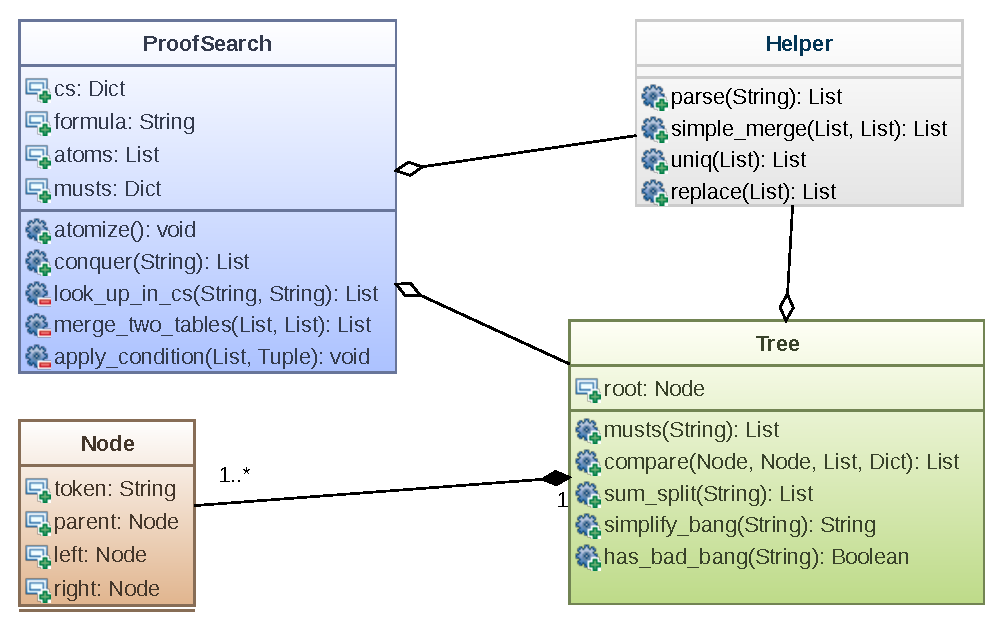
\includegraphics[width=0.9\textwidth]{/home/lyriael/BA/j-logic/thesis/Figures/uml_01.pdf}
	\caption{Simplified UML graphic of the classes used for implementing the algorithm. The list of methods and attributes is by no means complete and should simply give an idea of the construction.}
	\label{uml}
\end{figure}

\section{Operation Syntax Tree}
One of the earliest challenges was a useful representation of a formula with which I could work decently. Interestingly enough a binary tree came only later into my mind, after I tested various libraries from Python. There were libraries that seemed very useful at first as they were math-specific. Analyzing formulas that contained $*$ or $+$ were fairly easy but as $:$ and $!$ are not very common operations I could not customize the tested libraries enough to handle those as well.

So it happened while I was searching yet for another library that I tumbled over the possibility to use binary trees to represent the syntax of a mathematical formula. Remembering a lot of what I learned in the lecture about Datastructure and Algorithms I realized that this is the best choice for me. A binary tree gives me not only a way to represent a formula in a way that interprets the order of operations but with the knowledge about trees it became suddenly very easy to also manipulate such a formula for example by deleting or swapping subtrees and still keep a valid operation. 

I decided to implement my own tree for that purpose. It might be argued that a lot of work could be saved if I used available syntax trees but for one thing I relished the idea of implementing a tree structure that I would use myself and thus finally use what I have learned in lecture ages ago and second I would have to make custom changes to a finished solution anyway and those changes are probably more work than the implementation of a binary tree which is rather simple.

I tried to keep the tree as simple as possible, giving the nodes only a value and not a unique key. The greatest challenge given by implementing a syntax tree was to handle the unary operator $!$. As braces serve to determine the depth of a tree and a binary operation tells you when to start climbing up again, it required so extra case handling for the $!$ operator. From the point on when the tree was working, it was not only important to the algorithm, but could also be used to check if the input was written correctly. Therefore most of the tests that test the string handling of a tree are the result of formulas used somewhere else but which needed syntax spell checking. 


\section{Important Methods}
In this section I want to show and explain some of the more complicated methods that are important and make up the heart of the algorithm.

\subsection{Tree.musts}
The method \emph{musts} expects a given proof term to be already \emph{atomized} as it only distinguishes between $!$ and $*$ operations.
The algorithm takes the formula in form of a tree apart from top to bottom, generating new, smaller terms for every operation it takes apart until the remaining proof term is only a proof constant. Since the resolve of a $*$ operation needs a new \emph{X-wild} and the resolve of a $!$ operation replaces an existing \emph{x-wild} and therefore needs a new as well, the current $i$ for a new \emph{X-wild} $X_i$ is stored and increased in \texttt{v\_count}.

\begin{figure}[H]
    \vspace{-10pt}
	\lstinputlisting[firstline=2, lastline=22]{/home/lyriael/BA/j-logic/thesis/code_tree.py}
	\vspace{-10pt}
	\caption{Excerpt from $Tree.musts$}
	\vspace{-10pt}
\end{figure}

If for example the current justification term would be $((a*(!b)):F)$, it would be taken apart to the two subformulas $(a:(X_i\rightarrow F))$ and $((!b):(X_i))$. Because of the \emph{atomization} in the steps before it is guaranteed that every $!$ is a (right) child of a  $*$ and since every $*$ creates a new $X_i$, a term here that starts with a $*$ is always on a $X_i$. Since from $!b:X_i$ follows $\exists X_j \quad s.t. \quad !b:(b:X_j)$, all $X_i$ that occurred up to now must be replaced by $(b:X_j)$. In the end we will have only proof constants remaining.

\subsection{Tree.compare}
This method gives us foundation to the method \emph{apply\_condition} which we will look at later. It is also only very tedious and was probably written and rewritten again more than any other part of the code. It basically compares the value of each node of a tree with the corresponding value of a node of another tree. As long as the token (value) of the nodes are the same it will just process, but in case the two nodes are not identical several cases will be distinct.


\begin{figure}[H]
	\vspace{-10pt}
	\lstinputlisting[firstline=24, lastline=38]{/home/lyriael/BA/j-logic/thesis/code_tree.py}
	\vspace{-10pt}
\end{figure}
\begin{figure}[H]
	\vspace{-10pt}
	\lstinputlisting[firstline=41, lastline=46]{/home/lyriael/BA/j-logic/thesis/code_tree.py}
	\vspace{-10pt}
	\caption{Excerpt from $Tree.compare$}
	\vspace{-10pt}
\end{figure}

If the current node of the term from the cs-list has a \emph{Y-wild} all other occurrences of this \emph{Y-wild} within this term will be replaces with whatever node or subtree is found in the term of the \emph{musts}. As a consequence it is possible to find a \emph{X-wild} within the term from the cs-list. Whenever that is the case, the value found in the node/subtree of the term of the \emph{musts} is a condition to this $X_i$. If the condition is merely a constant value, it will be set directly.

As can be seen here the return value of this method is a list of conditions and a dictionary containing the found wilds. If a contradiction is found during the comparison both will be set to \texttt{None} rather than being returned empty, since it is possible that a comparison need neither conditions nor wilds but still works.
\todoWriteMore{Graphic with wild replacement for compare method}

\subsection[ProofSearch.apply\_conditions]{ProofSearch.apply\_condition \\and ProofSearch.apply\_all\_conditions}
These methods are called from within the method \texttt{full\_merge\_of\_two\_configs} if the wilds of the configurations can be merged. It is used to make sure that the new found configuration still holds for all conditions that applied before to each of the old configurations before they were merged.

This again proved more difficult than expected so I split it in two methods where the first simply handles one condition on one term and the other method makes sure that all conditions are taken care of. In the cases I studied so fare there is usually only one condition to a configuration but since it is possible that a configuration holds several conditions the method must hold in those cases as well.

\subsubsection{Apply One Condition}
The input arguments given to the method are the merged configuration and one condition tuple.

\begin{figure}[H]
	\vspace{-10pt}
	\lstinputlisting[firstline=1, lastline=3]{/home/lyriael/BA/j-logic/thesis/code_proof_search.py}
	\vspace{-10pt}
	\caption{Excerpt from $ProofSearch.apply\_condition$.}
	\vspace{-10pt}
\end{figure}

Since a condition is always on one $X_i$ the term we find in the configuration for $X_i$ is of high interest. But because the condition term may also contain other $X_j$ we need the whole configuration and not only the term on which the condition is. If there is now term for $X_i$ in the configuration yet the condition cannot be applied and must be kept for later reference. 

In the case that we do find an entry for $X_i$ in the configuration it will be compared with what we have in the condition term.

\begin{figure}[H]
	\vspace{-10pt}
	\lstinputlisting[firstline=8, lastline=25]{/home/lyriael/BA/j-logic/thesis/code_proof_search.py}
	\vspace{-10pt}
	\caption{Excerpt from $ProofSearch.apply\_condition$.  }
	\vspace{-10pt}
\end{figure}

Generally spoken there are three outcomes for a condition when it is checked against the merge of two configurations.

\begin{itemize}
	\item The condition is in contradiction with the merge of the two configurations. The merge is abandon and not further considered.
	\item The condition holds against the new merge but a comparison gave use \emph{X-} and/or \emph{Y-wilds}.
	\begin{itemize}
		\item Found \emph{X-wilds} will be written into the configuration merge.
		\item Found \emph{Y-wilds} will be passed on to be handled later on.
	\end{itemize}
	\item The condition holds against the new merge and no \emph{wilds} emerged. The condition is discarded since it is not used anymore.
\end{itemize}

\subsubsection{Apply All Conditions}
Applying all conditions instead of just one should be straight forward but I found it more difficult than expected. Since the number of conditions may change during iteration and since it is also possible that a condition that held a \emph{Y-wild} can change and has to checked again, a simple \texttt{loop} would not do.

\begin{figure}[H]
	\vspace{-10pt}
	\lstinputlisting[firstline=36, lastline=58]{/home/lyriael/BA/j-logic/thesis/code_proof_search.py}
	\vspace{-10pt}
	\caption{Excerpt from $ProofSearch.apply\_condition$. The  }
	\vspace{-10pt}
\end{figure}


If the condition can be satisfied the variable \texttt{updated\_config} will be true for the \texttt{if}-query. If a condition is still returned it must be kept for later reference thus. If \texttt{Y-wilds} contains any entries all conditions that contain any of the wilds (even those that have been checked already) will be updated and checked again. This is for the case that a \emph{Y-wild} has been found and although a \emph{Y-wild} may stand for any term, it must be the same term for all $Y_i$. 

The \texttt{break} in the code indicates the situation that one of the conditions could not be satisfied thus the whole merge is a fail. 

\subsection[ProofSearch.merge]{ProofSearch.full\_merge\_of\_two\_configs \\and merge\_two\_tables}
Similar as in the previous section the process that uses the methods above and actually merges all configurations together to get a solution is split in two parts where the first part handles a merge of only two configurations and the other handles the full merge.

\subsubsection{Simple Merge}
The actual merge is a very simple method found in the \texttt{Helper} class. It simply checks if the two given lists contain the same \texttt{String} or if at least one of the items in the list is an empty \texttt{String}.

\subsubsection{Full Merge of Two Configs}


\section{Tests}
\todoWriteMore{Todo}


\chapter{Example}
\label{chap: Example}
%!TEX root = ../bachelors_thesis.tex
\begin{example}
\[
	((((a*b)*(!b))+((!b)+c))+((!b)*d)):(b:F)
\]
\end{example}

%\newpage{\pagestyle{empty} \cleardoublepage}
%
%\input{Content/guidedImageFiltering}
%
%\newpage{\pagestyle{empty} \cleardoublepage}

\chapter{Conclusion}
%!TEX root = ../bachelors_thesis.tex
\todoWriteMore{Todo}
\section{Application}
\section{Enhancement}

 
%\addcontentsline{toc}{chapter}{\numberline{}List of Tables}
%\listoftables

%\addcontentsline{toc}{chapter}{\numberline{}List of Figures}
%\listoffigures
\addcontentsline{toc}{chapter}{\numberline{}Bibliography}
\bibliographystyle{plain}
%\bibliographstyle{plain}
\bibliography{sources}
%\bibliographystyle{alphadin}
\nocite{*}

\newpage{\pagestyle{empty} \cleardoublepage}
%\chapter*{Authorship}
%\listoftodos

\end{document}